\chapter{Устройство гитары}
\label{ch:guitar}

Частота от звука к звуку повышается в \emph{геометрической} прогрессии. То есть частота каждого следующего музыкального звука в \[\sqrt[12]{2}\approx 1,059463\] больше частоты звука предыдущего.

Так, следующий за ЛЯ первой октавы, звук ЛЯ-диез, имеет частоту $440\cdot\sqrt[12]{2}\approx 466,16$ герц. Звук СИ имеет частоту $440\cdot(\sqrt[12]{2})^2\approx 493,88$. И так далее, например, ЛЯ второй октавы имеет, как и положено, в два раза большую частоту, чем ЛЯ первой октавы: $440\cdot(\sqrt[12]{2})^{12}=440\cdot 2=880$ Гц.

Задав эталонную частоту любого музыкального звука, частоты для всех остальных звуков можно \emph{вычислить}.


TODO: ноты на грифе

\section{Устройство гитары}
\label{ch:guitar:construction}

Мы разобрались с теорией нот в предыдушем разделе, теперь коснемся особенностей устройства гитары, которые позволяют извлекать ноты именно такими, какими они и должны быть. 

Для начала стоит взглянуть на рисунок \ref{fig:guitar:construction} и запомнить, что значат незнакомые вам обозначения.

\begin{figure}[!ht]
    \centering
    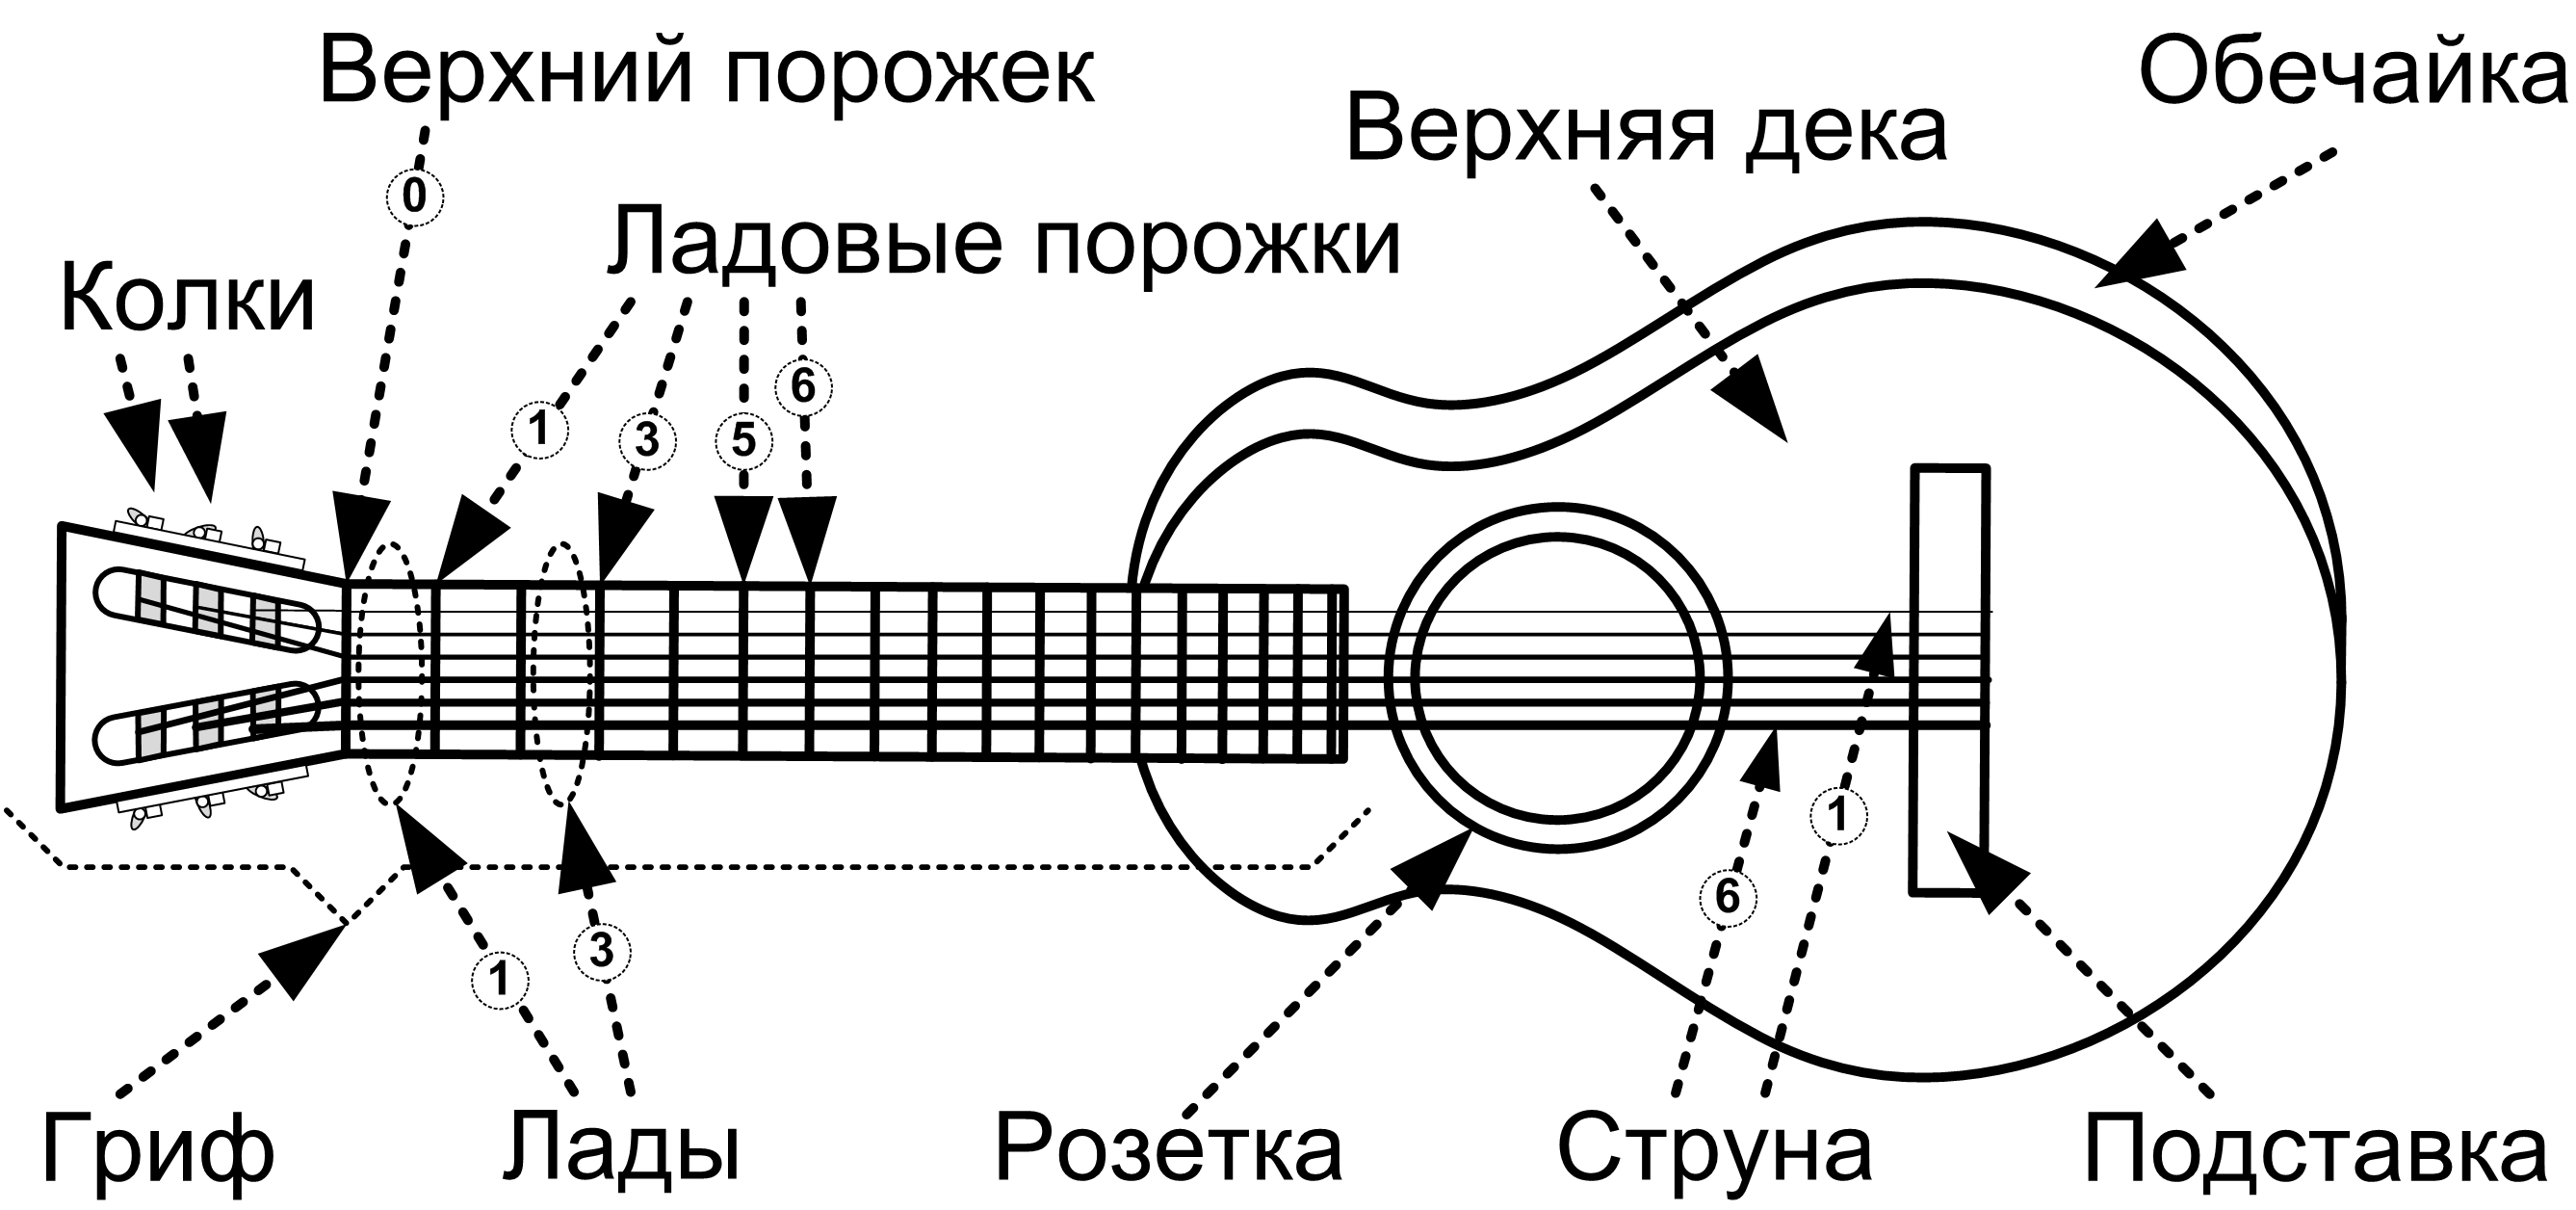
\includegraphics{fig/guitar-construction} 
    \caption{Устройство гитары}\label{fig:guitar:construction}
\end{figure} 

Любая открытая\footnote{То есть не зажатая ни на каком ладу} струна гитары звучит строго определенной нотой (о настройке гитары поговорим позже). Лады на грифе (промежутки между порожками), равно как и \emph{ладовые порожки} считаются от \emph{верхнего} порожка: 1,2,3,\ldots и т.д. То есть <<зажать струну на первом ладу>> значит, что вы ставите палец на струну, на первый лад, то есть между верхним порожком и первым ладовым\footnote{Чем ближе к первому ладовому, тем лучше. Таким образом и звук будет чище, и рука уставать будет меньше. Ставить палец сверху на порожек не стоит --- звук будет <<глохнуть>>. Правда иногда именно это и требуется. Но в начале обучения стоит ставить палец на ладу ближе к тому порожку, от которого идет <<звучащая>> часть струны. Добивайтесь чистого звука.} и нажимаете до тех пор, пока струна не прижмётся к первому ладовому порожку. Но нам важно сейчас не то, как правильно зажимать струну. 

Важно понять, что каждый следующий лад повышает звук на струне на <<полутон>>. В октаве 12 нот и каждая звучит на струне на своём ладу. На дветадцатом ладу звучит нота открытой струны, только выше на октаву.

Из физики известно, что частота колебаний струны обратно пропорциональна её длине\footnote{Надо честно заметить, что частота колебаний струны зависит также и от силы её натяжения, которая меняется, когда струну <<зажимают>> на ладу. Но это влияние столь незначительно, что им можно пренебречь.}. Стало быть, чтобы частота издаваемого струной звука \emph{увеличилась} вдвое (а языком музыки --- чтобы нота зазвучала октавой выше), надо вдвое \emph{укоротить} струну. 

Зажимая струну на 12 ладу (языком музыки --- повышая ноту открытой струны на октаву), вы укарачиваете звучащую часть струны вдвое. Линейка в помощь, если не верите\footnote{Конечно нужно мерять только звучащую (колеблющуюся часть) струны от опоры на подставке до 12-го ладового порожка.}.

Конечно, частота колебаний струны зависит также и от силы её натяжения. Сила натяжения струны регулируется колками на грифе, когда гитару настраивают. Играя, гитарист только меняет длину звучащего участка струны, зажимая струны на ладах. Редкие психи\footnote{Конечно, имелось в виду: \emph{мастера}! Прим. ред.} крутят колок во время исполнения, добиваясь сомнительных\footnote{Конечно, имелось в виду: \emph{удивительных}! Прим. ред.} эффектов.

Исходя из того, что частота каждой следующей ноты в $\sqrt[12]{2}$ больше предыдущей, запишем формулу длины струны ($L$) от места крепления струны к подставке до $n$-го ладового порожка:

\[L(n)=\frac{L}{(\sqrt[12]{2})^n},\]
где $n$ - номер лада ($0$-й лад соответствует открытой струне), а $L$ --- общая длина струны от подставки до верхнего порожка.


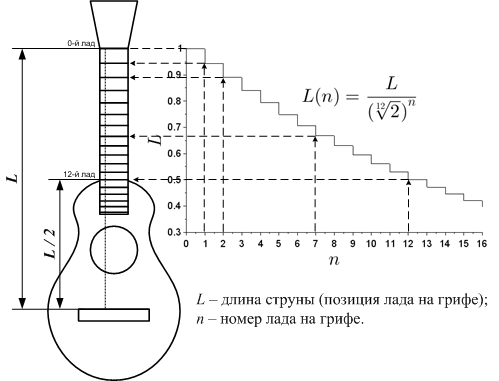
\includegraphics{fig/string-length.png}


Из картинки, надеюсь, ясно, почему ладовые порожки на гитаре расположены не на равном расстоянии друг от друга.

Кстати, некоторые ушастые выпендрёжники говорят, что различают своим сверхмузыкальным слухом больше 12 нот в октаве! И им мало 12 ладов! Есть спрос --- есть предложение: на некоторых гитарах можно заметить дополнительные ладовые порожки между <<каноническими>>, которые позволяют <<всунуть>> дополнительную ноту.


\section{Запись гитарных нот на бумаге}

Чтобы записать ноты, купите нотную тетрадь или на обычном листе начертите нотоносец --- пять параллельных, расположенных друг под другом через равные интервалы (около двух миллиметров) линий:
 

Традиционно ноты для шестиструнной гитаре записываются в скрипичном ключе, который своим хвостиком огибает вторую снизу линию нотоносца, на которой располагется Соль \emph{малой} октавы\footnote{Для других музыкальных инструментов, в первую очередь, для фортепиано, скрипичный ключ показывает положение Соль \emph{первой} октавы, но для гитары, чтобы использовать один нотоносец, ноты пишут на <<фортепианный>> скрипичный нотоносец на октаву выше.}.


\section{Поиск нот на грифе}

\begin{figure}[!ht]
    \centering
    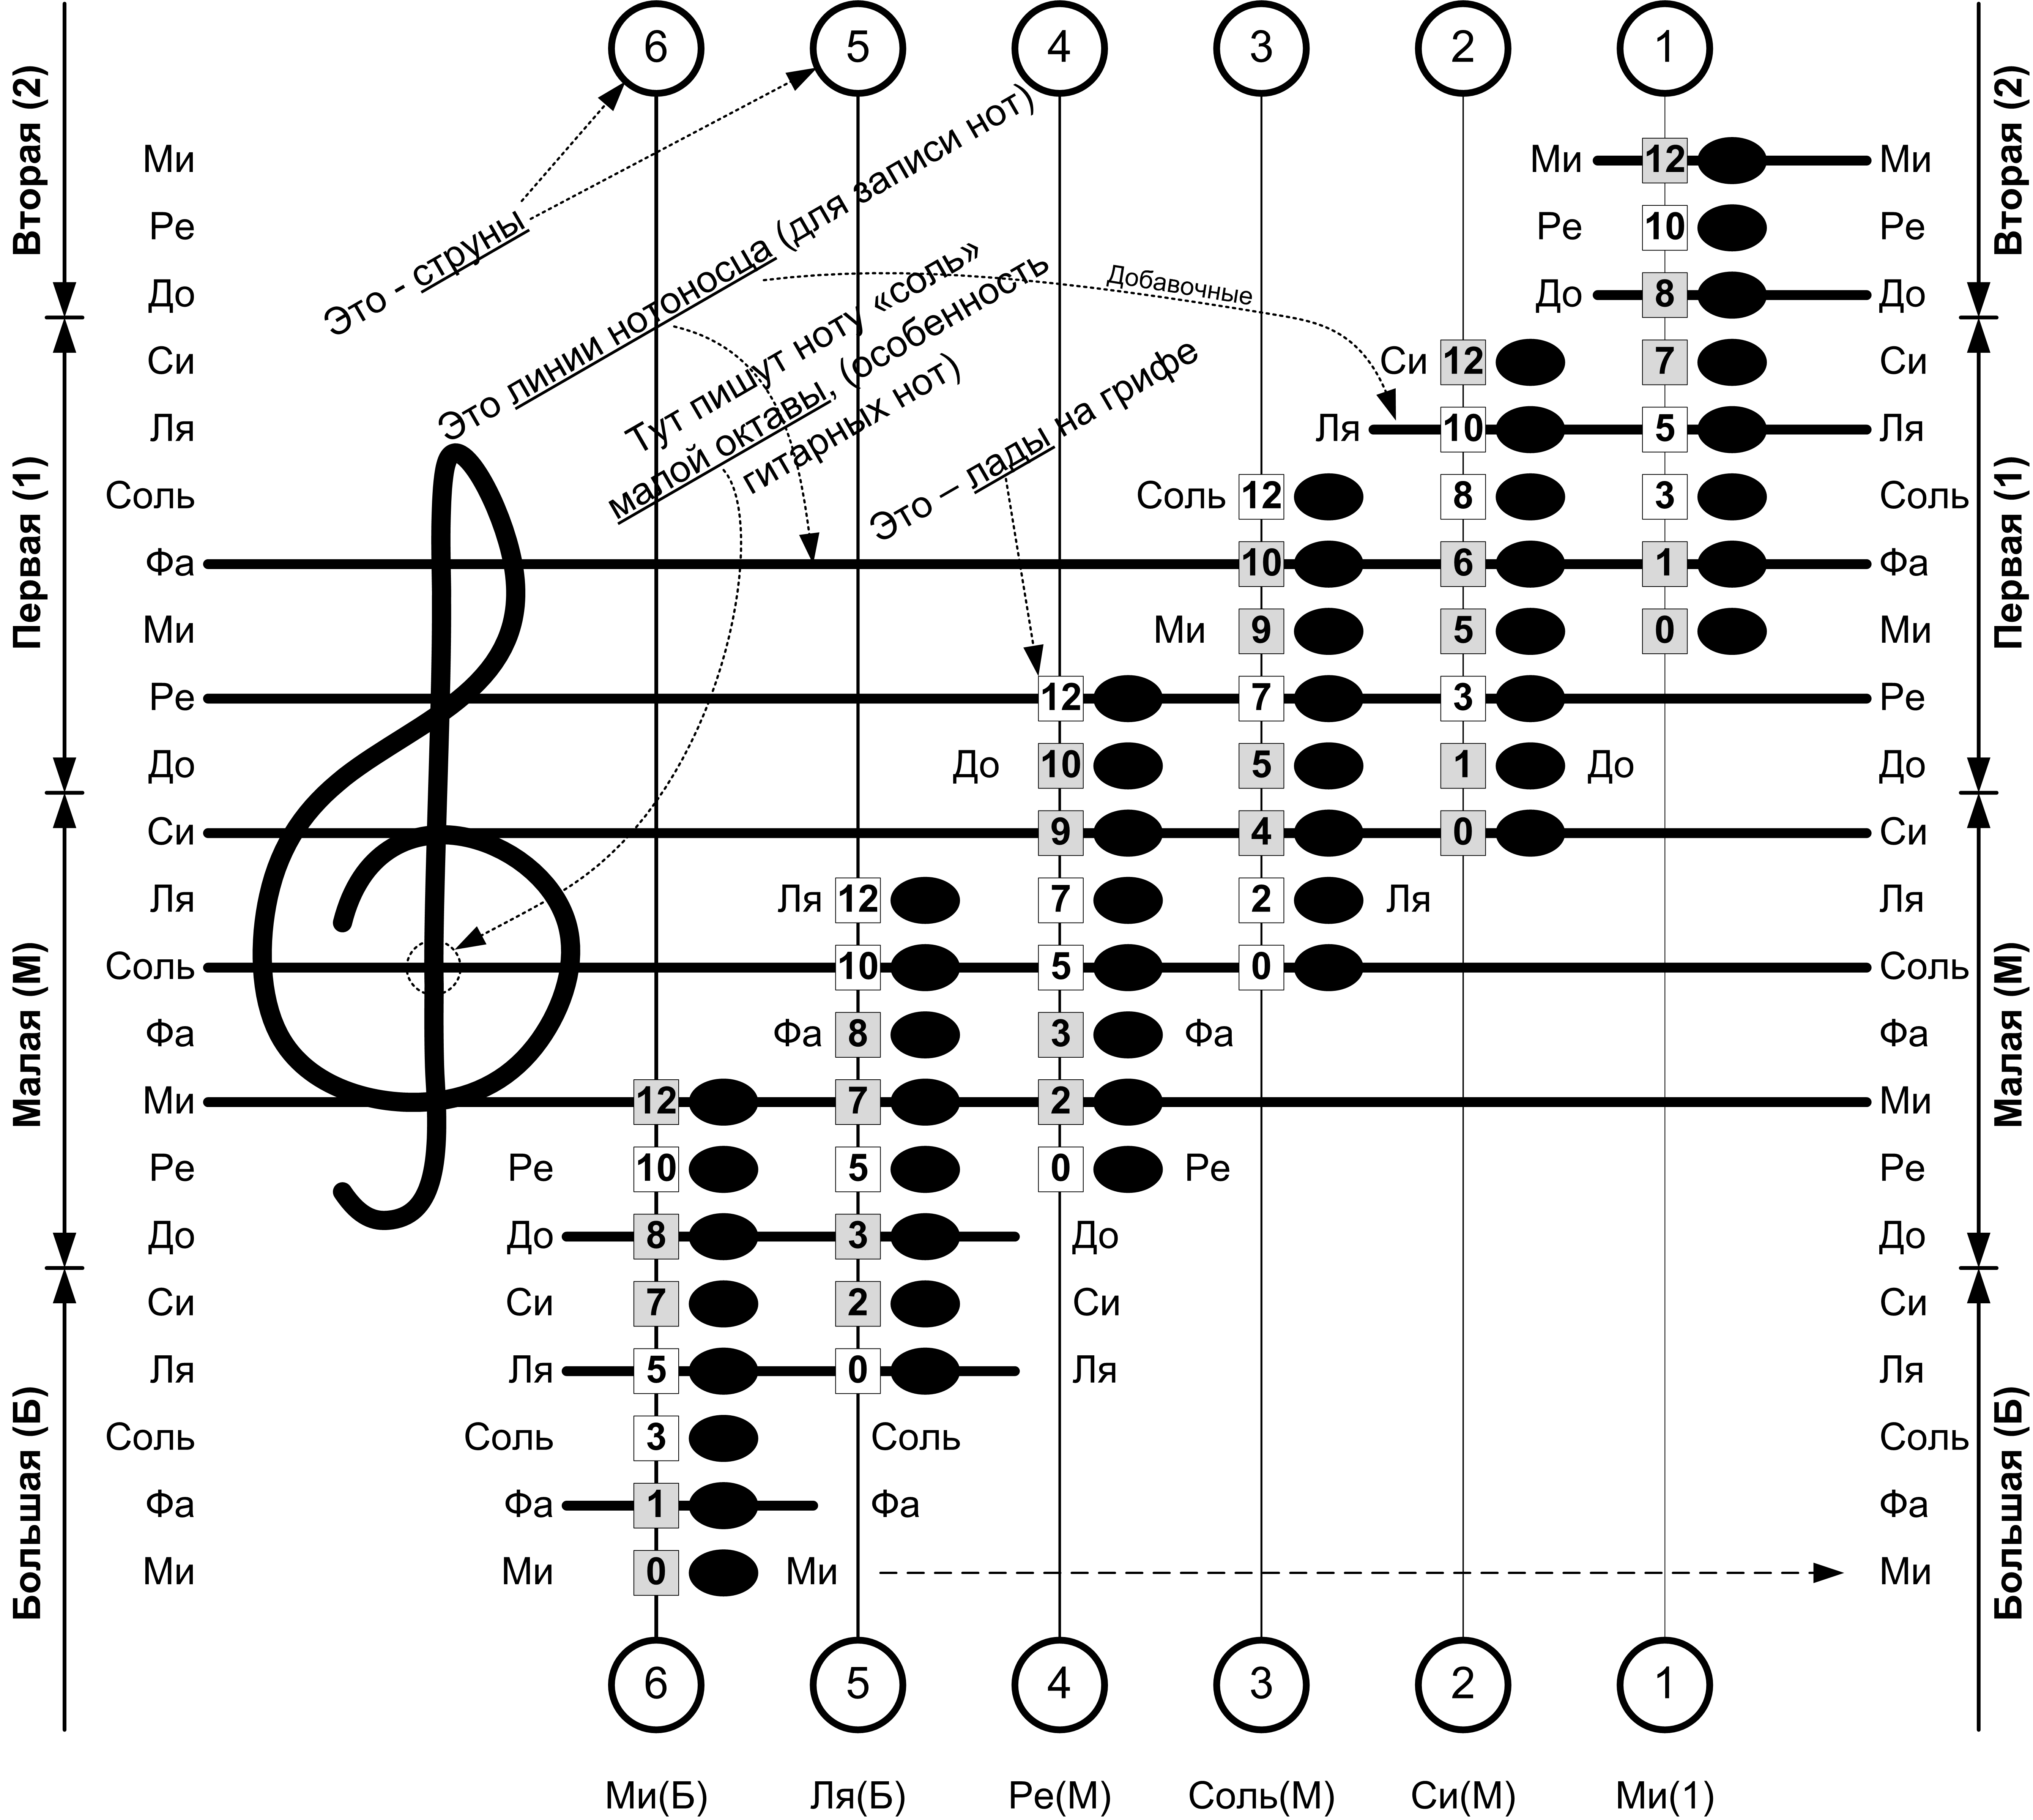
\includegraphics[width=\textwidth]{fig/lad-by-notes} 
    \caption{Ноты на грифе (гриф поперек нотоносца)}\label{fig:ladByNotes}
\end{figure} 

\begin{figure}[!ht]
    \centering
    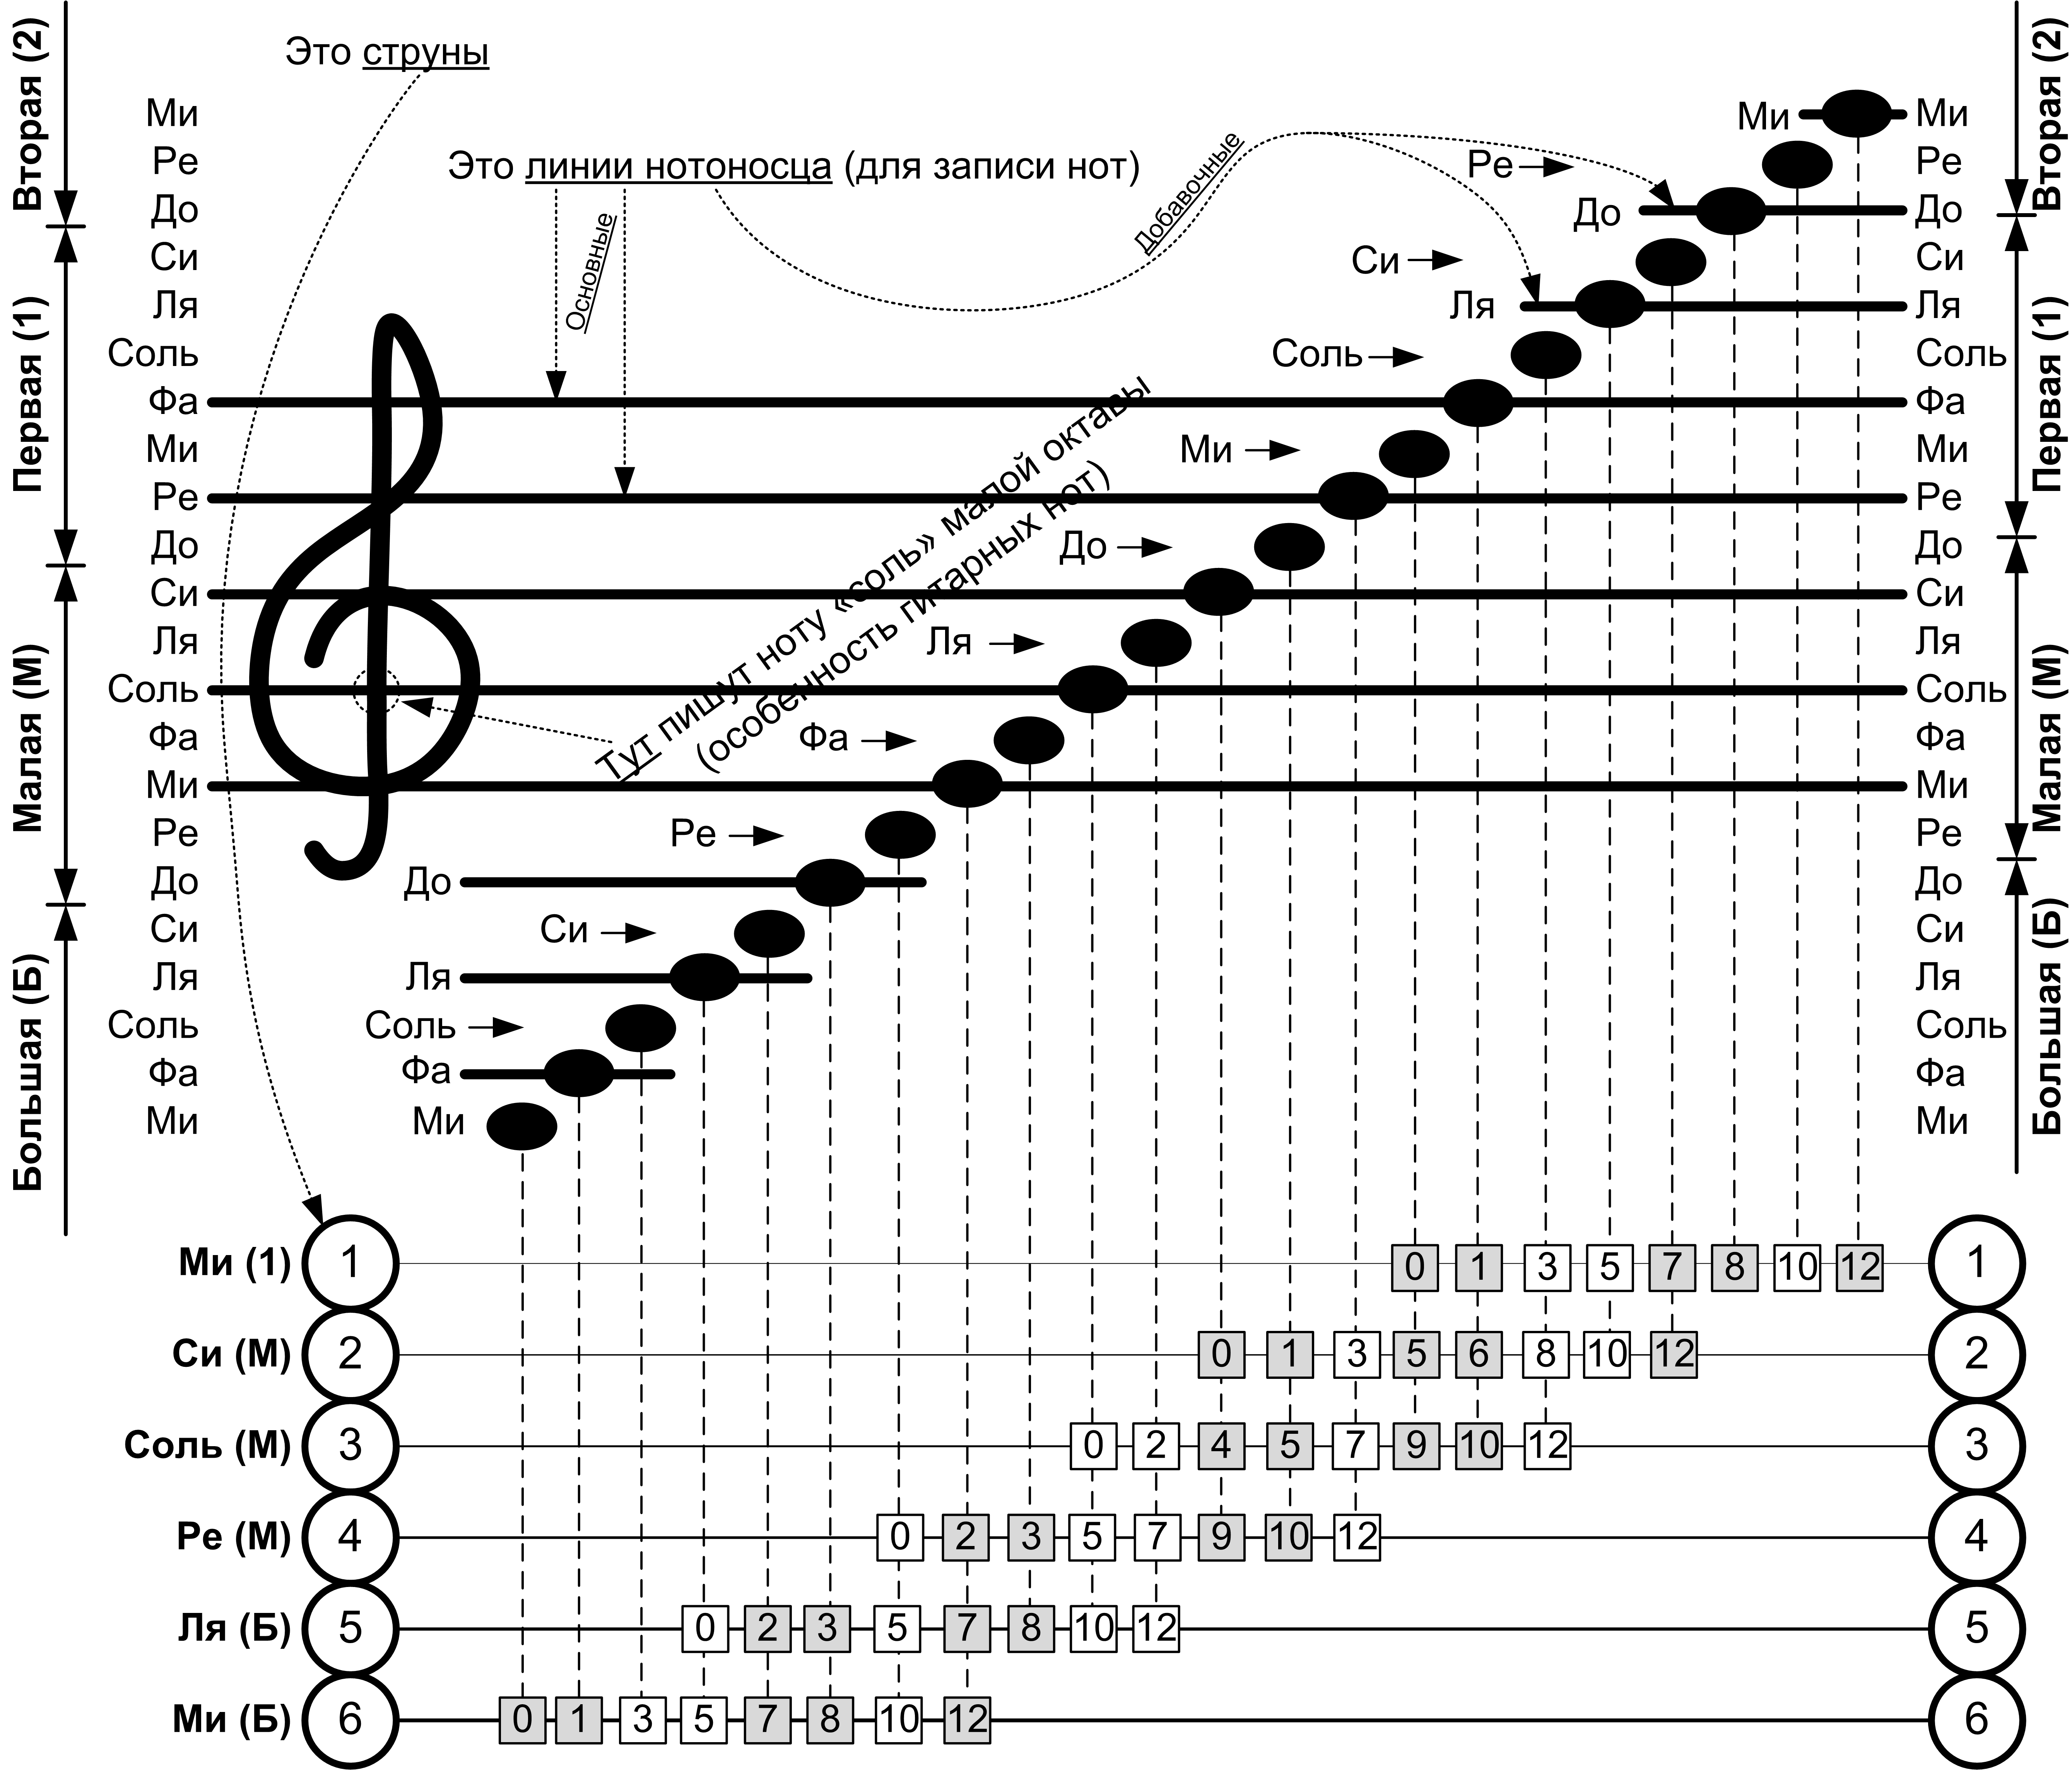
\includegraphics[width=\textwidth]{fig/lad-by-griph} 
    \caption{Ноты на грифе (гриф вдоль нотоносца)}\label{fig:ladByGriph}
\end{figure} 

\begin{figure}[!ht]
    \centering
    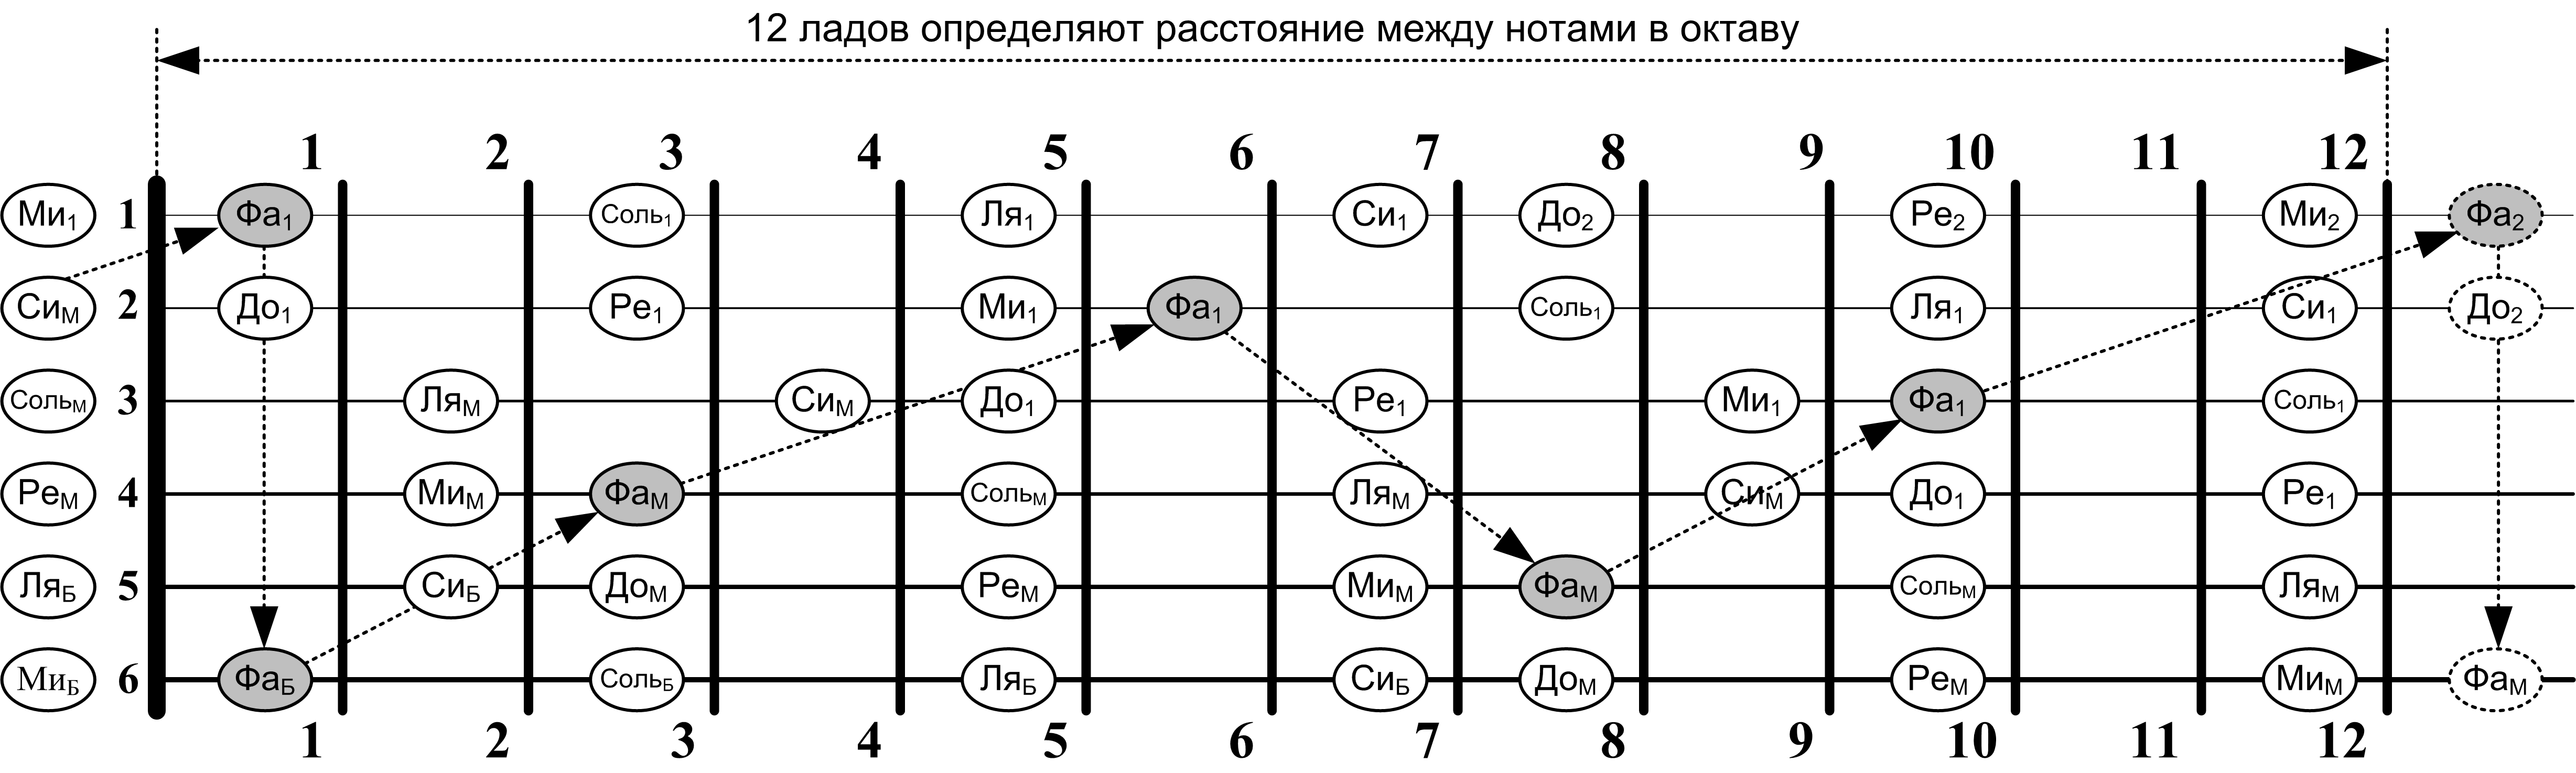
\includegraphics[width=\textwidth]{fig/notes-on-griph} 
    \caption{Ноты на грифе (относительное расположение)}\label{fig:notesOnGriph}
\end{figure} 


